\chapter{Implementacja}
Jak wspomniano w poprzednim rozdziale, dane wejściowe są wskazaniami pomiarów z~poszczególnych posterunków opadowych. Są to dane punktowe, zatem aby oszacować ilość wody jaka spadła na zadanym obszarze konieczne jest przeprowadzenie ich interpolacji w~celu aproksymacji wartości dla punktów stanowiących granicę wskazanej zlewni, co dalej zmierza do wyznaczenia opadu powierzchniowego.

Istnieje wiele metod wyznaczania średniego opadu powierzchniowego. Począwszy od prostego obliczenia średniej arytmetycznej wartości z~posterunków opadowych, poprzez metody wieloboków Voronoia, izohiet po hipsometryczną. Różnią się one dokładnością, sposobem aproksymacji czy też zaawansowaniem danych wejściowych.

Jak wspomniano we wstępie, praca ta traktuje o analizie danych pojedynczego opadu, a~nie zbieranych przez pewien okres czasu. Przy wyborze sposobu przekształcenia danych jest to bardzo istotne kryterium, które wraz z~możliwością jak najlepszego dopasowania do kształtu zlewni stanowiło główne wymagania tej części pracy.

%\section{Triangulacja i algorytm Delaunay'a}
%Do przeprowadzenia interpolacji danych punktowych zastosowano technikę triangulacji. Polega ona na stworzeniu siatki trójkątów o~wierzchołkach w punktach z~wartością znaną (wysokość opadu na posterunku opadowym). Wybór padł na zastosowanie algorytmu Delaunay'a, który wprowadza dodatkowe ograniczenie na tworzone trójkąty. Mianowicie, okrąg opisany na każdym z~nich nie może zawierać innych punktów siatki poza wierzchołkami danego trójkąta. Ta metoda ma na celu maksymalizację równoboczności powstałych trójkątów, a~co za tym idzie, równomierność budowanej siatki.

\section{Zastosowana metoda}
Wybór padł na połączenie techniki triangulacji wraz z~interpolacją przy użyciu płaszczyzny.

Triangulacja polega na stworzeniu siatki trójkątów o~wierzchołkach w~zadanych punktach (w tym wypadku są to posterunki opadowe o znanej wysokości opadu). Zastosowano algorytm Delaunay'a, który wprowadza dodatkowe ograniczenie na tworzone trójkąty. Mianowicie, okrąg opisany na każdym z~nich nie może zawierać innych punktów siatki poza wierzchołkami danego trójkąta. Ta metoda ma na celu maksymalizację równoboczności powstałych trójkątów, a~co za tym idzie, równomierność budowanej siatki.

\begin{figure}[ht]
	\centering
	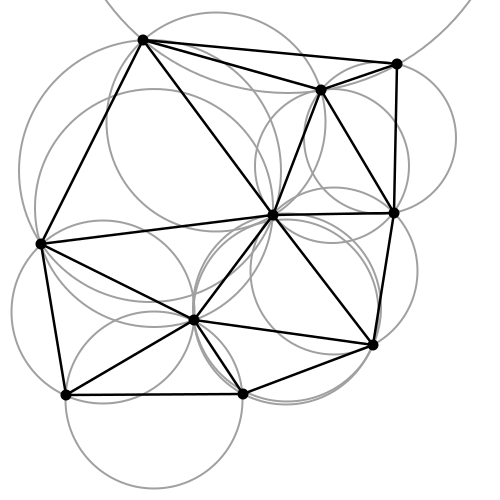
\includegraphics[scale=0.3]{delaunay}
	\caption{Schemat zastosowania algorytmu Delaunay'a (źródło: wikipedia)}
	\label{fig:delaunay}
\end{figure}

\begin{figure}[ht]
	\centering
\begin{subfigure}[t]{.5\textwidth}
	\centering
	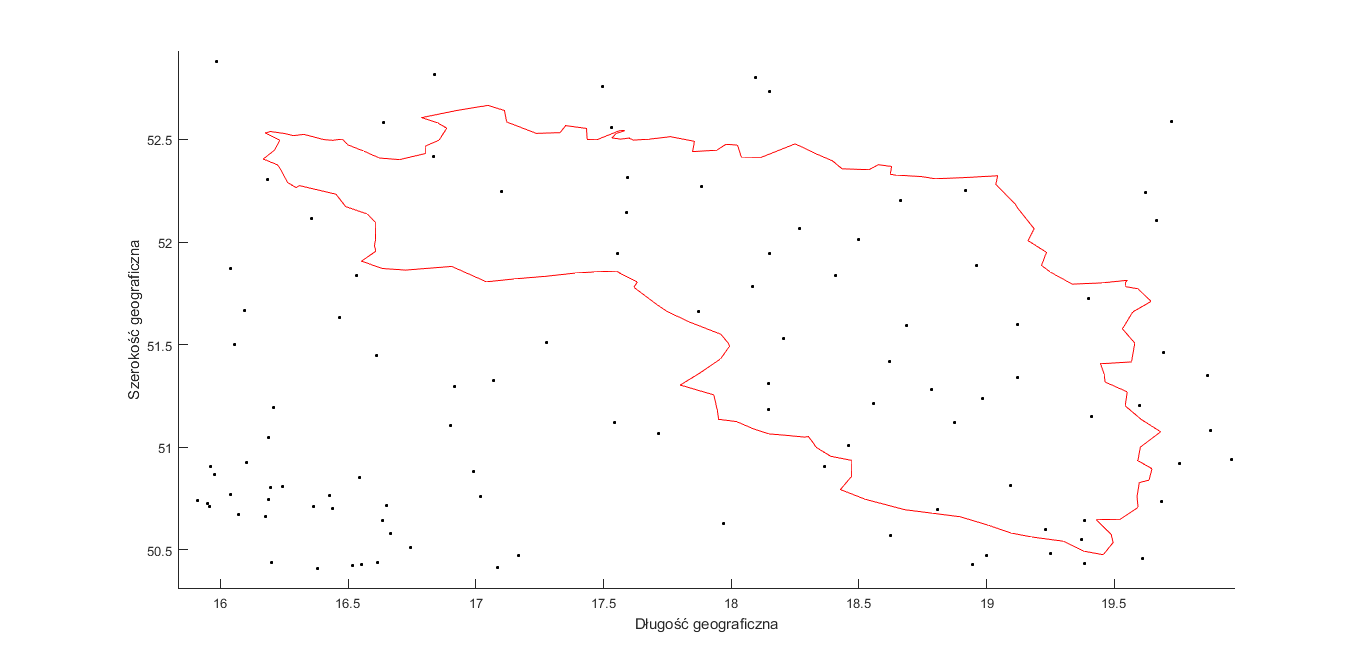
\includegraphics[width=0.7\linewidth]{dane_wejsciowe}
	\caption{Posterunki opadowe i~obszar zlewni}
	\label{fig:dane_wejsciowe}
\end{subfigure}	
	\begin{subfigure}[t]{0.5\textwidth}
	\centering
	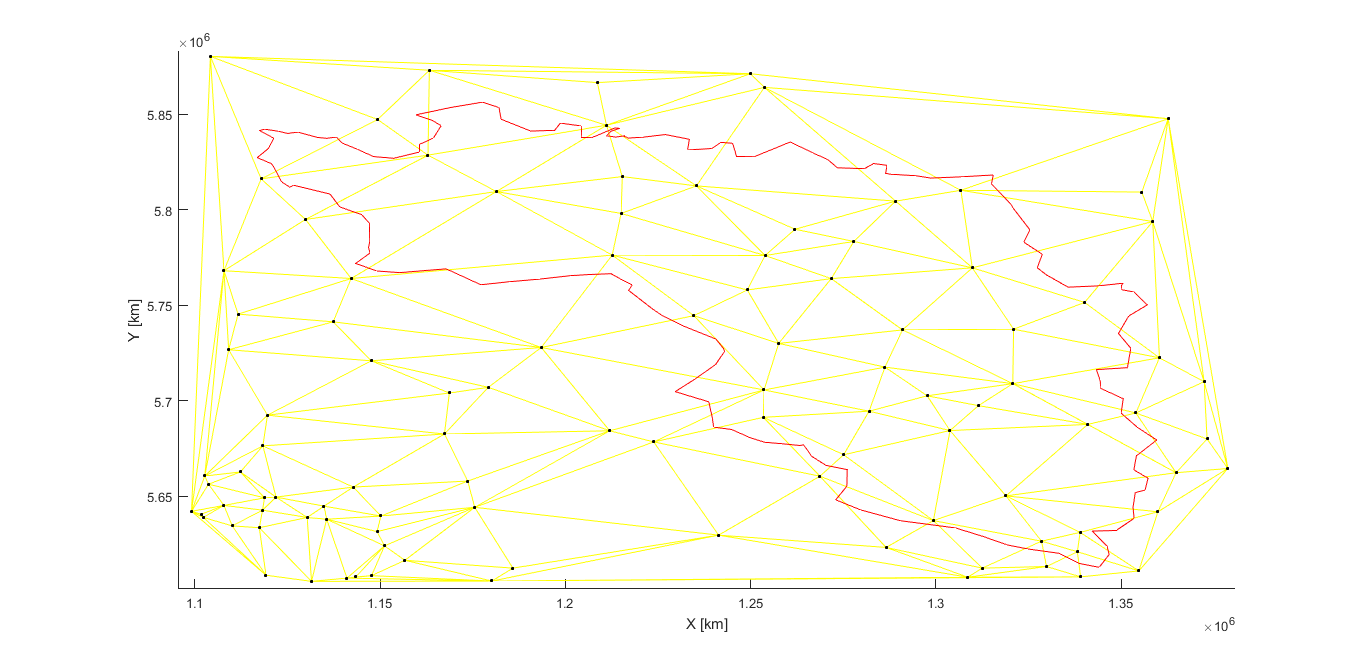
\includegraphics[width=0.7\linewidth]{triangulacja_zlewnia}
	\caption{Siatka triangulacji dla posterunków}
	\label{fig:triagnulacja_danych}
\end{subfigure}	
\caption{Prezentacja danych wejściowych}
	
\end{figure}

Po zastosowaniu triangulacji następnym etapem jest wyznaczenie punktów, dla których należy interpolować wartość opadu. Tymi punktami są poszczególne węzły granicy wskazanej zlewni oraz miejsca przecięcia tej granicy z krawędziami trójkątów. Wraz z~posterunkami opadowymi znajdującymi się wewnątrz obszaru dla jakiego wyznaczany jest obszar powierzchniowy będą stanowiły węzły kolejnej triangulacji.


\begin{figure}[ht]
	\centering
	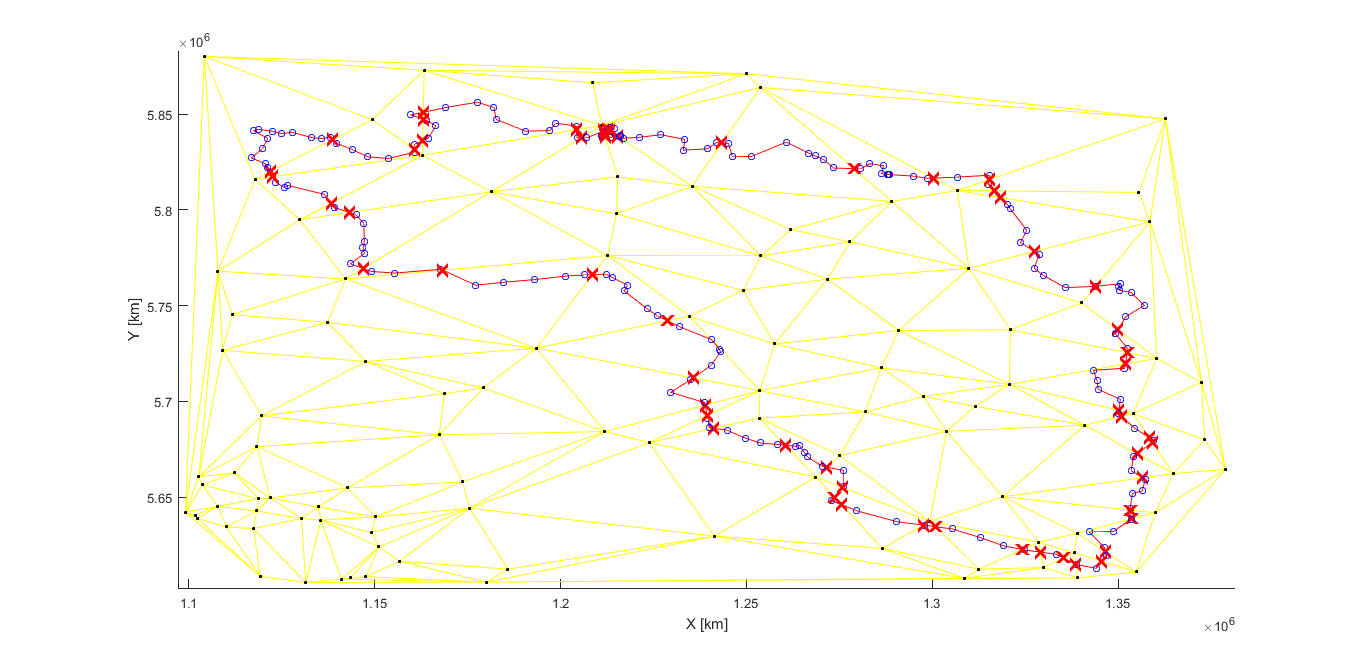
\includegraphics[scale=0.5]{punkty_do_interpolacji}
	\caption{Punkty wyznaczone do interpolacji.
	O - węzły granicy, X - przecięcia granicy z~liniami siatki.}
	\label{fig:punkty_interpolacji}
\end{figure}

Jak wspomniano na początku tego rozdziału, wyznaczenie wartości dla powstałych punktów odbywa się poprzez interpolację powierzchniową poszczególnych trójkątów.

Została stworzona funkcja wyznaczająca wektor normalny dla pojedynczego trójkąta. Wektor normalny jest prostopadły do powierzchni zadanej płaszczyzny. Z~jego pomocą (oraz znając współrzędne punktu należącego do płaszczyzny - np. jeden z~wierzchołków trójkąta) wyznacza się wartość \textit{z} punktu o~współrzędnych $x$~i~$y$~w~oparciu o~równanie ogólne płaszczyzny.

\begin{equation*}
\begin{gathered}
A(x - x_0) + B(y - y_0) + C(z - z_0) = 0 \\
[A, B, C] = (P_2 - P_1) \times (P_3 - P_2)
\label{eq:rownanie_plaszczyzny}
\end{gathered}
\end{equation*}
gdzie
% eqwhere z aghdpl powoduje błąd
\begin{description}[leftmargin=3cm, itemsep=0cm, labelsep=0cm]
	\item[$x_0, y_0, z_0$] współrzędne punktu należącego do płaszczyzny
	\item[$A, B, C$] współrzędne wektora normalnego
\end{description}

Przy użyciu przygotowanej funkcji, dla wszystkich wyznaczonych do interpolacji punktów uzyskiwana jest wartość opadu korzystając ze współrzędnych $x$~i~$y$ punktu i~wektora normalnego trójkąta, w~którym ten punkt się znajduje.

\begin{figure}[ht]
	\centering
	\includegraphics[scale=0.5]{algorytm}
	\caption{Schemat krokowy zastosowanej metody}
	\label{fig:algorytm}
\end{figure}

\begin{figure}[ht]
	\centering
	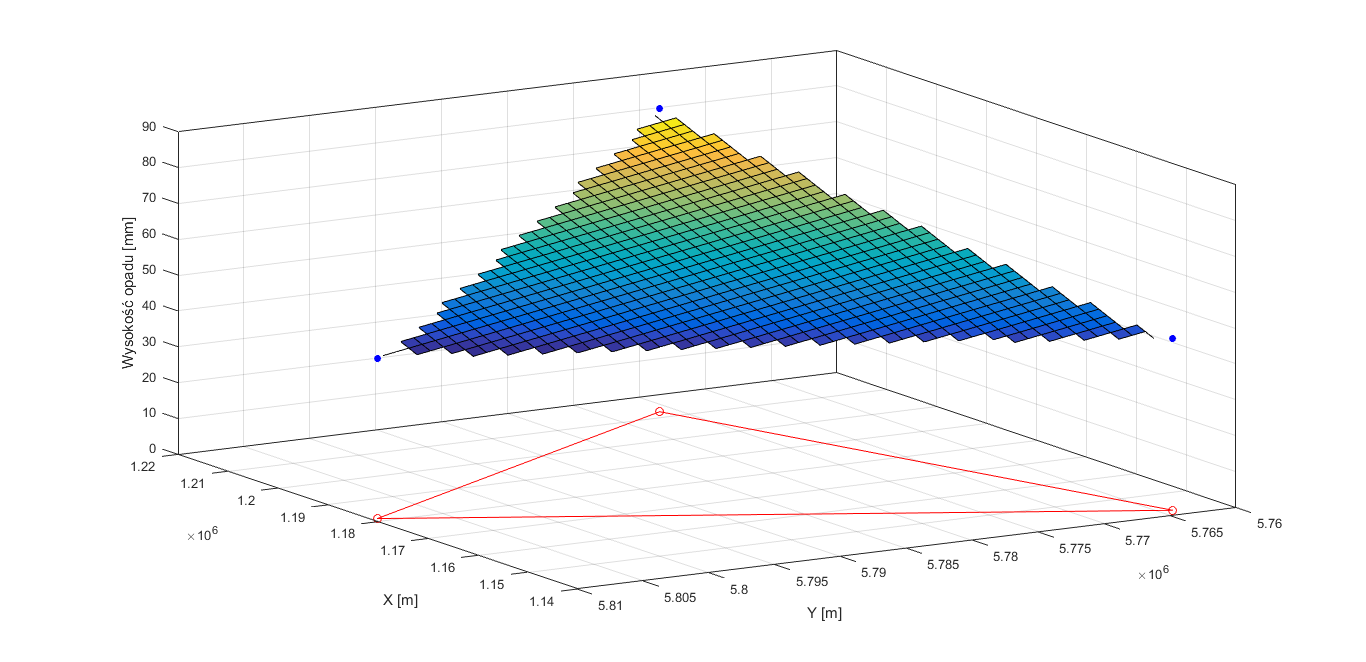
\includegraphics[scale=0.5]{prezentacja_interpolacji}
	\caption{Interpolacja płaszczyzną dla pojedynczego trójkąta}
	\label{fig:plaszczyzna_interpolacji}
\end{figure}

Po zakończeniu interpolacji wartości przeprowadzana jest ponowna triangulacja mająca na celu stworzenie brył o~trójkątnej podstawie (wysokości brył to wartość opadu w~punkcie będącym wierzchołkiem). Tym razem zastosowane zostaną punkty interpolowane oraz posterunki wewnątrz zlewni. Jak zaprezentowano na rysunku~\ref{fig:druga_triangulacja}, pojawia się komplikacja


\begin{figure}[ht]
	\centering
	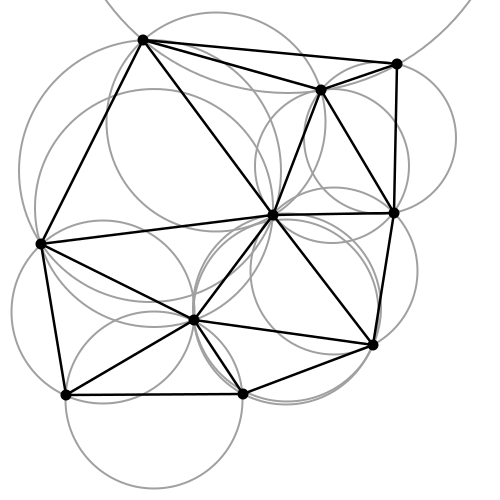
\includegraphics[scale=0.3]{delaunay}
	\caption{Schemat zastosowania algorytmu Delaunay'a (źródło: wikipedia)}
	\label{fig:delaunay}
\end{figure}

\begin{figure}[ht]
	\centering
\begin{subfigure}[t]{.5\textwidth}
	\centering
	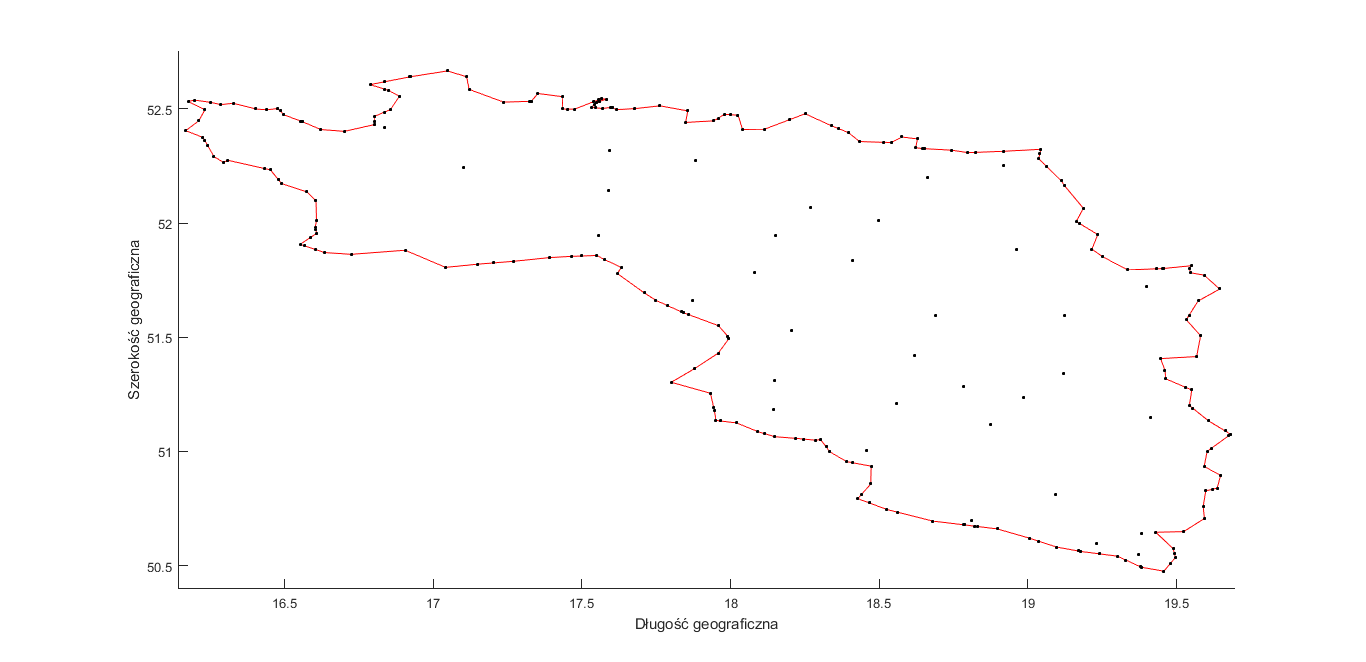
\includegraphics[width=0.7\linewidth]{dane_druga_triangulacja}
	\caption{Punkty dla ponownej triangulacji}
	\label{fig:dane_wejsciowe}
\end{subfigure}	
	\begin{subfigure}[t]{0.5\textwidth}
	\centering
	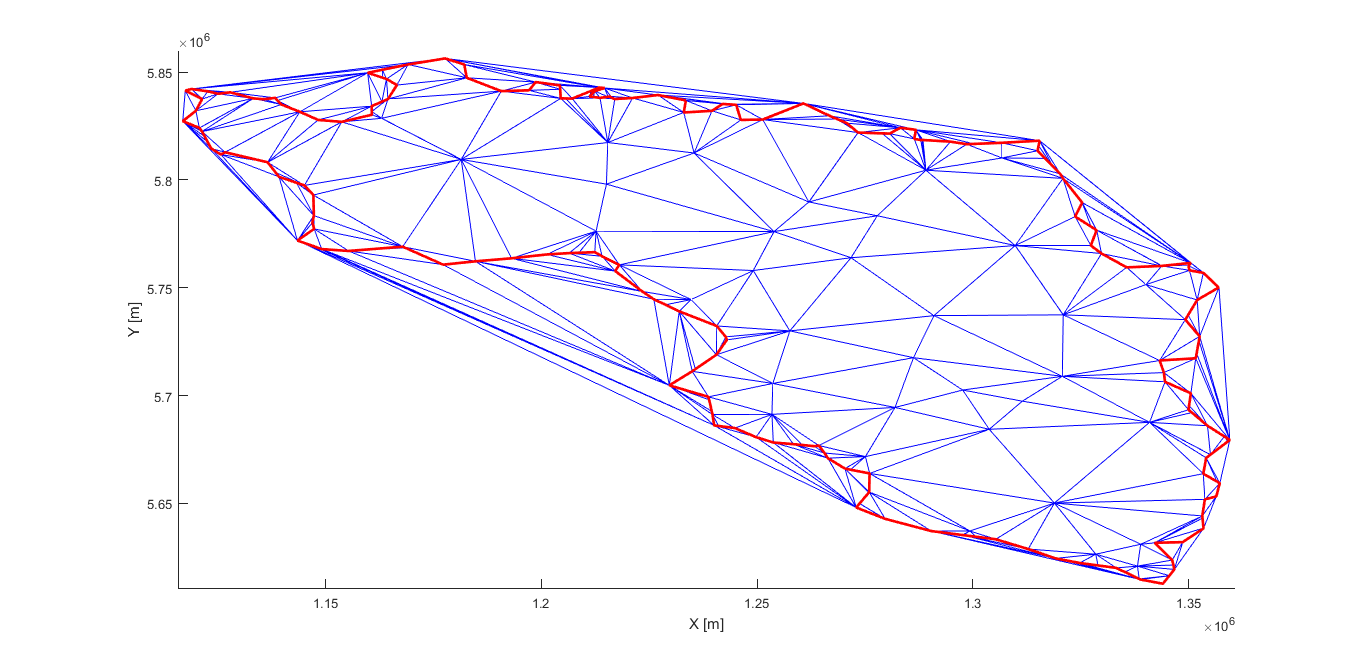
\includegraphics[width=0.7\linewidth]{druga_triangulacja}
	\caption{Siatka triangulacji dla wyznaczonych punktów}
	\label{fig:druga_triagnulacja}
\end{subfigure}	
\caption{Triangulacja danych interpolowanych}
	
\end{figure}